\documentclass{article}
\usepackage{assignment}

\lstset{
    language=Octave,
    frame=single,
    breaklines=true,
    title=\lstname,
}

\title{MAT4170 -- Assignment 2}
\author{Jon-Magnus Rosenblad}
\date{}

\begin{document}
\maketitle

\section*{Problem 1}
A B-simple of degree $d$ at a knot of multiplicity $n$ has smoothness $d - n$.
It is infinitely smooth outside the knots, i.e. on each open knot interval $(t_i,t_{i + 1})$,
and outside $[t_1, t_{d + 2}]$.
It follows that $B[0,0,0,0,1]$ has smoothness $3 - 4=-1$ and is in fact discontinuous at $0$,
and it has smoothness $3 - 1 = 2$ at $1$.
The other spline - $B[0,1,1,1,2]$ - has smoothness $3 - 1 = 2$ at $0$, $3 - 3 = 0$ at $1$, and $3 - 1 = 2$ at $2$.

\section*{Problem 2}

We claim that for any B-spline $B[t_1,\ldots,t_{d + 2}]$ of degree $d$
we have 

\begin{equation}
    B[t_1,\ldots, t_{d + 2}](t_i) = B[t_1,\ldots,\hat{t_i},\ldots,t_{d + 2}](t_i)
\end{equation}
where $\hat{t_i}$ means the knot $t_i$ is omitted.

We proceed by induction on the degree of $B$.
Using the convention that the degree zero B-spline $B[t_j,t_{j + 1}]$
is the indicator function for the interval $[t_j,t_{j + 1})$

\begin{equation}
    x\mapsto \begin{cases}
        1   &x\in [t_j, t_{j + 1})\\
        0   &\textrm{otherwise}.
    \end{cases}
\end{equation}

Observing that removing either knot from the either end of a linear spline
we end up with an interval not overlapping with the removed knot,
so the value will be $0$ in either case.
Removing the central knot we are at the top of the "hat" of the linear spline,
and for the degree zero spline we are somewhere in the interval spanned by the two other knots,
so the value will be $1$ in either case.

Some care needs to be taken in the case of knots with higher multiplicities,
but it is not difficult to see that the statement holds in this case as well.

Assume the claim holds for every spline of degree $d - 1$ with arbitrary knots.
Let $B[t_1,\ldots, t_{d + 2}]$ be a spline of degree $d$.
From the recursive definition of B-splines we have

\begin{equation} \label{eq:spline-recursion}
    B[t_1,\ldots, t_{d + 2}](x)
    = \frac {x - t_1}{t_{d + 1} - t_1}B[t_1,\ldots,t_{d + 1}](x)
    + \frac {t_{d + 2} - x}{t_{d + 2} - t_2}B[t_2,\ldots,t_{d + 2}](x).
\end{equation}

The edge-cases of $t_i=t_1,t_{d + 2}$ are easy by the fact that the splines evaluate to zero
outside the interval spanned by their knots, and we get the equality directly from the remaining 
summand of \autoref{eq:spline-recursion}.
For internal knots the inductive step follows from the inductive argument applied to both summands.

In the case that $t_i$ has higher multiplicity the interior- and edge-case coincide,
but we have a special case when $t_i$ has multiplicity $d + 1$.
It is resolved by the convention $0/0=0$ and the equality follows from the remaining summand. 

\section*{Problem 3}

\lstinputlisting{src/findKnotInterval.m}

\section*{Problem 4}

\lstinputlisting[label=alg:evaluateSpline]{src/evaluateSpline.m}
\lstinputlisting{src/plotSplines.m}

\begin{figure}
    \centering
    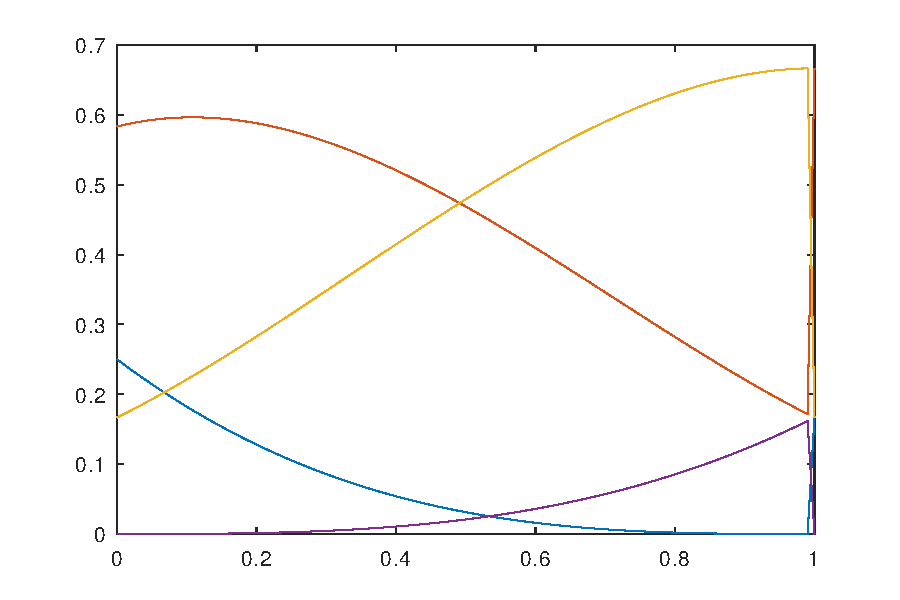
\includegraphics[width=\linewidth]{figures/plotSplines.pdf}
    \caption{The four degree $3$ polynomials. The distortion at $1$ is due to the relevant points being shifted by $1$.}
\end{figure}

\section*{Problem 5}

\lstinputlisting{src/computeSplinePoint.m}
\lstinputlisting{src/plotSplineCurve.m}

\begin{figure}
    \centering
    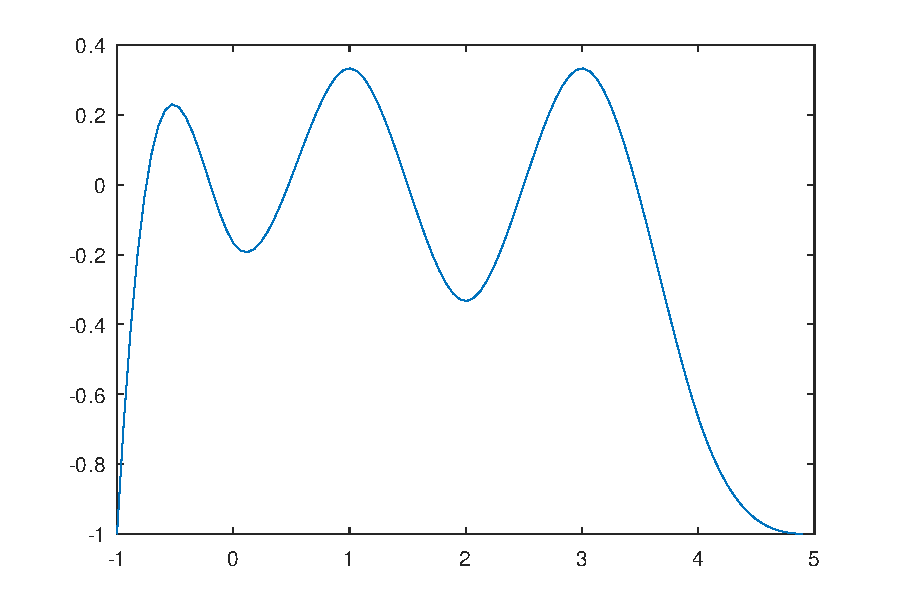
\includegraphics[width=\linewidth]{figures/plotSplineCurve.pdf}
    \caption{The spline curve of alternating coefficients in the interval [0,1]}
\end{figure}

\section*{Problem 6}

We may in fact compute the cubic spline by stitching together the different splines
evaluated ta the unit intervals $[i,i + 1]$ for $i=0,1,2,3$ using \hyperref[alg:evaluateSpline]{\texttt{evaluateSpline}}.
\lstinputlisting{src/plotWholeCubic.m}

\begin{figure}
    \centering
    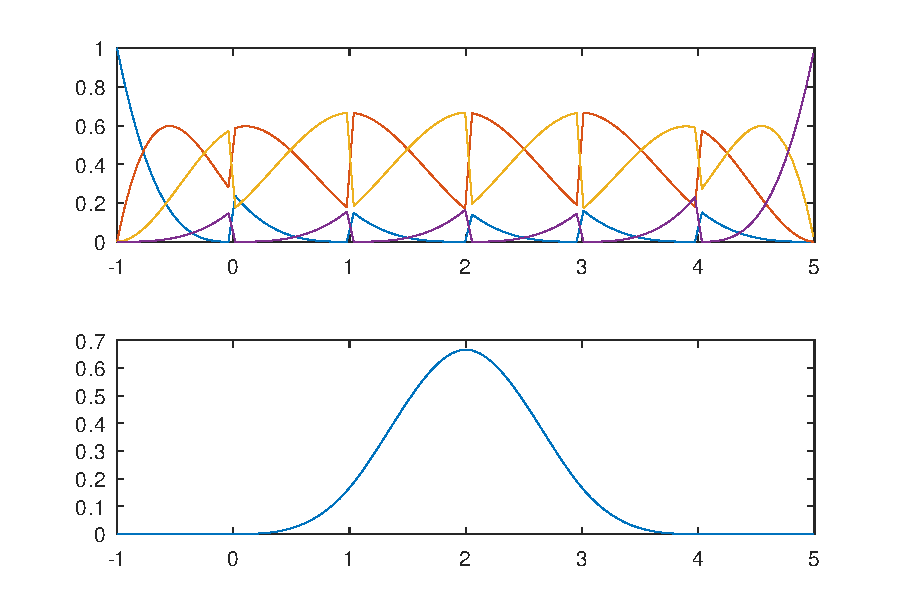
\includegraphics[width=\linewidth]{figures/plotWholeCubic.pdf}
    \caption{The stitched version of the B-splines on the different intervals.}
\end{figure}

\end{document}
